\documentclass[../../FisicaTeorica.tex]{subfiles}

%%%PACKAGES
\usepackage[usenames, dvipsnames, table]{xcolor}
\usepackage[utf8]{inputenc}
\usepackage[T1]{fontenc}
\usepackage{lmodern}
\usepackage{amsmath}
\usepackage{amsthm}
\usepackage{amsfonts}
\usepackage{comment}
\usepackage{wrapfig}
\usepackage{booktabs}
\usepackage{braket}
\usepackage{pgf,tikz}
\usepackage{mathrsfs}
\usetikzlibrary{arrows}
\usepackage{subfigure}
\usepackage{xspace}
\usepackage{gnuplottex}
\usepackage{epstopdf}
\usepackage{marginnote}
\usepackage{float}
\usetikzlibrary{tikzmark}
\usepackage{graphicx}
\usepackage{cancel}
\usepackage{bm}
\usepackage{mathtools}
\usepackage{hyperref}
\usepackage{ragged2e}
\usepackage[stable]{footmisc}
\usepackage{enumerate}
\usepackage{mathdots}
\usepackage[framemethod=tikz]{mdframed}
\PassOptionsToPackage{table}{xcolor}
\usepackage{soul}
\usepackage{enumerate}
\usepackage{mathdots}
\usepackage[framemethod=tikz]{mdframed} %Added 16/10
\usepackage[italian]{babel} %Added 16/10
\usepackage{amssymb} %Added
\usepackage{enumitem}
\usepackage{array}


%%BOOKTAB
\setlength{\aboverulesep}{0pt}
\setlength{\belowrulesep}{0pt}
\setlength{\extrarowheight}{.75ex}
\setlength\parindent{0pt} %Rimuove indentazione


%%GEOMETRIA
\usepackage[a4paper]{geometry}
 \newgeometry{inner=20mm,
            outer=49mm,% = marginparsep + marginparwidth 
                       %   + 5mm (between marginpar and page border)
            top=20mm,
            bottom=25mm,
            marginparsep=6mm,
            marginparwidth=30mm}
\makeatletter
\renewcommand{\@marginparreset}{%
  \reset@font\small
  \raggedright
  \slshape
  \@setminipage
}
\makeatother
 

%%COMANDI
\newcommand{\q}[1]{``#1''}
\newcommand{\lamb}[2]{\Lambda^{#1}_{\>{#2}}}
\newcommand{\norm}[1]{\left\lVert#1\right\rVert}
\newcommand{\hs}{\mathcal{H}}
\newcommand{\minus}{\scalebox{0.75}[1.0]{$-$}}
\newcommand{\hlc}[2]{%
  \colorbox{#1!50}{$\displaystyle#2$}}
\newcommand{\bb}[1]{\mathbb{#1}}
\newcommand{\op}[1]{\operatorname{#1}}
\renewcommand{\figurename}{Fig.}
\newcommand{\dom}[1]{D#1}
\newcommand{\avg}[1]{\left\langle{#1}\right\rangle}
\newcommand{\NN}{\mathbb N}
\newcommand{\RR}{\mathbb R}
\newcommand{\CC}{\mathbb C}
\newcommand{\mS}{\mathcal S}
\newcommand{\de}{d}
\newcommand{\abs}[1]{\left|#1\right|}

\newcommand{\lesson}[2]{\marginpar{(Lezione #1 del #2)}}
\DeclareRobustCommand{\MQ}{{\small\textsc{MQ}}\xspace}
\DeclareRobustCommand{\MC}{{\small\textsc{MC}}\xspace}
%Prima era \small\textsc{MQ}\xspace

%%TESTATINE
\usepackage{fancyhdr}
\pagestyle{fancy}
\fancyhead{} % clear all header fields
\renewcommand{\headrulewidth}{0pt} % no line in header area
\fancyfoot{} % clear all footer fields
%\fancyfoot[R]{A.A. 2018/19} % other info in "inner" position of footer line
\cfoot{\thepage}


%%AMBIENTI
\theoremstyle{plain}
\newtheorem{thm}{Teorema}[section]
\newtheorem{lem}{Lemma}[section]
\newtheorem{prop}{Proposizione}[section]
\newtheorem{axi}{Assioma}
\newtheorem{pst}{Postulato}

\theoremstyle{definition}
\newtheorem{dfn}{Definizione}

\theoremstyle{remark}
\newtheorem{oss}{Osservazione}
\newtheorem{es}{Esempio}
\newtheorem{ex}{Esercizio}

%Spiegazioni/verifiche
\newenvironment{expl}{\begin{mdframed}[hidealllines=true,backgroundcolor=green!20,innerleftmargin=3pt,innerrightmargin=3pt,leftmargin=-3pt,rightmargin=-3pt]}{\end{mdframed}} %Box di colore verde

\newenvironment{appr}{\begin{mdframed}[hidealllines=true,backgroundcolor=blue!10,innerleftmargin=3pt,innerrightmargin=3pt,leftmargin=-3pt,rightmargin=-3pt]}{\end{mdframed}} %Approfondimenti matematici (box di colore blu)

%%Domande di Marchetti
\newtheorem{question}{Domanda}


%%OPERATORI
\DeclareMathOperator{\sech}{sech}
\DeclareMathOperator{\csch}{csch}
\DeclareMathOperator{\arcsec}{arcsec}
\DeclareMathOperator{\arccot}{arcCot}
\DeclareMathOperator{\arccsc}{arcCsc}
\DeclareMathOperator{\arccosh}{arcCosh}
\DeclareMathOperator{\arcsinh}{arcsinh}
\DeclareMathOperator{\arctanh}{arctanh}
\DeclareMathOperator{\arcsech}{arcsech}
\DeclareMathOperator{\arccsch}{arcCsch}
\DeclareMathOperator{\arccoth}{arcCoth} 




\begin{document}
\section{L'operatore momento}
\subsection{Momento in $\bb{R}$}
\begin{center}
    \small{(18-19/10/2018)}
\end{center}
Consideriamo l'operatore momento $P=-i\hbar \frac{d}{dx}$ "a dominio reale", cioè su $\hs = L^2(\bm{\bb{R}}, dx)$. Esaminiamone nel dettaglio il dominio, espandendo tutte le condizioni che avevamo prima sintetizzato con una semplice "regolarità".\\
In particolar modo, è necessario chiedere che:
\begin{itemize}
    \item Esista la derivata $\psi'$ \textit{quasi ovunque}.
    \item Poiché dovremo fare un'\textit{integrazione per parti}, ci serve che $\psi' \in L^2(\bb{R}, dx)$ e sia "integrabile alla Lebesgue su ogni compatto":
    \[
    \int_a^b \psi'(x)dx = \psi(b)-\psi(a)\>\forall [a,b]\in \bb{R}
    \]
\end{itemize}
\textbf{Nota}: È necessario che le condizioni siano così "larghe". Per esempio, potremmo essere tentati di sintetizzarle chiedendo che $\psi \in C^1$. Ciò, tuttavia, fa perdere l'autoaggiuntezza dell'operatore, e perciò fa sì che il suo spettro non sia più solamente reale!\\
Definiamo perciò il dominio di $P$ come:
\begin{align*}
D\left(P\right)= \big\{\psi\in L^2\left(\mathbb{R},\ dx\right)\ \ |\ \ 
&\exists\psi^\prime\ q.o.\, \int_{a}^{b}{\psi^\prime\left(x\right)dx}=\psi\left(b\right)-\psi\left(a\right)\ \forall\left[a,b\right]\in\mathbb{R},\\
&\psi^\prime\in L^2(\mathbb{R},\ dx)\ \big\}
\end{align*}
\textbf{Nota}: per \textit{definire} un operatore è necessario indicarne in maniera esplicita il dominio. Come vedremo tra poco, infatti, lo "stesso operatore" su domini diversi può dar luogo a risultati assurdi, o essere associato a diverse osservabili.\\

Fissate queste condizioni, si ha subito che se $\psi$ , $\psi^\prime\in L^2(R, dx)$ allora $\psi(x)$ si annulla all'infinito:
\[
\lim_{x\rightarrow\pm\infty}{\psi\left(x\right)}=0
\]
A priori non è nemmeno ovvio che tale limite esista. Potremmo per esempio considerare una funzione che si annulla ovunque, se non in determinati intervalli (di misura non nulla), in cui "salta" a un certo valore positivo. Calibrando opportunamente la larghezza dei "salti" e distanziandoli tra loro si può far sì che l'integrale di tale $\psi$ converga a un valore finito - e quindi che $\psi \in L^2$. Tuttavia, poiché tali "salti" sono sempre presenti, per quanto grande sia $M$, per $x>M$ la funzione assume valori che non si avvicinano a $0$ più del valore del "salto", e perciò il limite a $\infty$ non esiste.\\
Tuttavia, se $\psi$ e $\psi' \in L^2(\bb{R})$, allora lo sono anche su $\mathbb{R}_+$: $\psi$,$\psi^\prime\in L^2([0, +\infty [, dx)$. Ma allora:
\[
\int_0^\infty dx (\psi^*(x)\psi'(x)+{\psi^*}'(x)\psi(x)) = \int_0^\infty dx \frac{d}{dx}(\psi^*(x), \psi(x)) = \norm{\psi(\infty)}^2 - \norm{\psi(0)}^2
\]
e tale integrale esiste finito perché abbiamo richiesto sia possibile l'integrazione per parti.\\
Ma allora esiste $\norm{\psi(\infty)}$, e quindi anche:
\begin{equation}
\psi(\infty) = \lim_{x\to\infty} \psi(x) = 0
\label{eqn:psitozero}
\end{equation}
(Se fosse qualsiasi altro valore eccetto $0$ si avrebbe che $\psi \notin L^2$).\\

Verifichiamo allora l'autoaggiuntezza $P = P^\dag$. Essendo $D(P)$ denso in $\hs$ partiamo dall'uguaglianza degli elementi di matrice per definire $P^\dag$ e osservare quali condizioni è necessario imporre per il suo dominio:
\[
\left(\phi,P\psi\right)=(P^\dag\phi,\psi); \quad \forall \phi \in D(P^\dag);\> \forall \psi \in D(P)
\]
Calcolando il prodotto scalare:
\[
\int_{-\infty}^{+\infty}{dx\,\phi^\ast\left(x\right)\left[\hlc{SkyBlue}{-i\hbar\frac{d}{dx}\psi\left(x\right)}\right]\underset{(a)}{=}
\hlc{Yellow}{-i\hbar\phi^\ast\left(x\right)\psi\left(x\right)\big|_{-\infty}^{+\infty}}+\int{\left[\hlc{SkyBlue}{-i\hbar\frac{d}{dx}\phi\left(x\right)}\right]^\ast\psi\left(x\right)dx}}
\]
(dove in (a) si è integrato per parti).\\
Se il termine evidenziato in giallo si annullasse avremmo dimostrato che l'aggiunto $P^\dag$ ha la stessa forma di $P$, ossia che $P$ è simmetrico (le espressioni corrispondenti a $P$ e $P^\dag$ sono evidenziati in azzurro). Sappiamo che tale termine si annulla poiché, come visto in (\ref{eqn:psitozero}), $\psi(x)$ si annulla all'infinito. Tale conclusione è però valida solamente se l'integrazione per parti effettuata in (a) è sensata, ossia se anche per $\phi$ valgono le richieste che abbiamo fatto per $\psi$ a tal proposito, e cioè che $\phi'$ esista quasi ovunque, $\phi, \phi' \in L^2(\bb{R},dx)$ e $\phi'$ Lebesgue-integrabile su compatti.\\
Ma allora le condizioni che abbiamo imposto per trovare $D(P)$ sono esattamente le stesse che caratterizzano $D\left(P^\dag\right)$, e quindi:
\[
D\left(P\right)=D(P^\dag)
\]

\subsection{Momento in $\bb{R}_+$}
Paradossalmente, se cerchiamo di restringere la definizione di $P$ ai soli reali positivi, ossia ponendo $\hs=L^2\left(\mathbb{R}_+,\ dx\right)$, la costruzione di prima non porta ad alcun operatore autoaggiunto. Verifichiamolo.\\
Sia $P= -i\hbar \frac{d}{dx}$, e fissiamo:
\[
D\left(P\right)= \left\{\psi\in L^2\left(\mathbb{R}_+\right)\ |\ \exists\> \psi'
\text{ q.o. e sia definita l'integrazione per parti}, \psi^\prime\in L^2(\mathbb{R}_+)\right\}
\]
Ripetendo gli stessi passaggi di prima, si arriva a dover definire le condizioni per cui il primo termine dell'integrazione per parti (quello evidenziato in giallo nel caso precedente) si annulli:
\[
\phi^*(x)\psi(x)\big|_{0}^{+\infty} = \cancel{\phi^*(+\infty)\psi(+\infty)} - \phi^*(0)\psi(0) = 0
\]
Il problema è che dalle condizioni che abbiamo imposto finora sappiamo solo che $\psi$ si annulla all'infinito, ma nulla si sa sul suo comportamento in $0$. È quindi necessario imporre un'altra condizione - ma non c'è modo di farlo in maniera "simmetrica". Se infatti risolvessimo ponendo $\psi(0) = 0$ non dovremmo fare la stessa richiesta per la $\phi$ (non sarebbe necessario), e quindi $D(P) \subset D(P^\dag)$. Viceversa, se imponessimo $\phi(0) = 0$ avremmo la situazione opposta, con $D(P) \supset D(P^\dag)$.\\
Perciò, se richiediamo che il momento $P$ nell'intervallo $\bb{R}_+$ sia simmetrico, allora non può essere autoaggiunto, e quindi \textit{non è un'osservabile}.\\
Qual è il significato fisico di ciò?\\
ipotizziamo per assurdo che $P$ su $\bb{R}_+$ sia un'osservabile. Allora avremo degli autovalori, per esempio $p$ autovalore di $P$. Facendo quindi una misura del momento troveremmo allora $p$, e sapremmo per certo che $p>0$.\\
Con un'analogia semiclassica, "fissare un momento" significa considerare un'onda piana\footnote{Pensandola con il principio di indeterminazione: l'onda piana ha estensione infinita - quindi non conosciamo la sua posizione con nessuna precisione - ma ha un \textit{unico} momento $p$}. Tuttavia, un'onda piana "confinata" a $\bb{R}_+$ vuol dire che "si è riflessa" sul piano per $x=0$, ed è quindi in realtà la sovrapposizione di un'onda incidente e una riflessa - che hanno momenti di segno opposto\footnote{In altre parole, facendo oscillare una fune "infinitamente lunga" ma collegata ad un punto fisso - oltre il quale non c'è più nulla, e che corrisponde all'\textit{estremo del dominio}, ossia $x=0$, si crea un'\textit{onda stazionaria}, che classicamente si ottiene come sovrapposizione di due onde con verso opposto di propagazione}. Perciò anche in questo caso non è possibile ottenere una misura univoca del momento - e infatti l'operatore $P$ su $\bb{R}_+$ non corrisponde a osservabili.

%%19-10
\subsection{Momento in $[0,2\pi]$}
È invece possibile definire l'operatore momento su $[0,2\pi]$, cioè ponendo $\hs = L^2([0,2\pi],dx)$.\\
Nella costruzione del suo dominio inizialmente consideriamo un operatore "test" $\tilde{P}$, che poi raffiniremo al $P$ vero e proprio. Poniamo quindi:
\[
D\left(\widetilde{P}\right)= \left\{\psi\in L^2\left(\left[0,2\pi\right],dx\right)\ \ |\ \ \psi\text{ regolari},\psi\left(0\right)=\psi\left(2\pi\right)=0\right\}
\]
Ma $\widetilde{P}$ così definito non può essere autoaggiunto, poiché $D(\widetilde{P})\subset D({\widetilde{P}}^\dag)$. Infatti, partendo come prima dalla condizione di simmetria:
\[
\left(\widetilde{P}\phi,\psi\right)=\left(\phi,\widetilde{P}\psi\right)\quad \phi\in D(\tilde{P}^\dag), \> \psi \in D(\tilde{P})
\]
quando si giunge all'integrazione per parti, il primo termine il primo termine (quello evidenziato in giallo all'inizio) si annulla solamente per la condizione che abbiamo imposto sulle $\psi$:
\[
\phi^\ast\left(x\right)\psi\left(x\right)\big|_0^{2\pi}=0
\]
Ma allora sulle $\phi$ non serve imporre nulla oltre alla regolarità:
\[
D\left({\widetilde{P}}^\dag\right)=\left\{\phi\in L^2\left(\left[0,2\pi\right],dx\right)\ |\ \phi\text{ regolari}\right\}
\]
da cui $D(\tilde{P})\subset D(\tilde{P}^\dag)$.\\
In effetti $\tilde{P}$ non produce risultati fisici. Risolvendo infatti l'equazione agli autovalori (per separazione delle variabili):
\begin{align*}
    &\tilde{P}\ket{\lambda} = \lambda \ket{\lambda} \Rightarrow -i\hbar\frac{d}{dx}\psi_\lambda = \lambda\psi_\lambda \Rightarrow \frac{\psi_\lambda'}{\psi_\lambda} = \frac{i\lambda}{\hbar}\\
    &\Rightarrow \ln \psi_\lambda = \frac{i\lambda}{\hbar}x + c \Rightarrow \psi_\lambda\left(x\right)=A e^{-i\frac{\lambda}{\hbar}x}
\end{align*}
Quando si impone (come richiesto dalle condizioni sul dominio di $\tilde{P}$) che $\psi_\lambda\left(0\right)=0$ si ottiene solo una funzione nulla - che non ha senso fisico.\\
La ragione intuitiva per cui ciò non funziona è che, come nel caso di $\mathbb{R}_+$, una situazione semiclassica in cui il momento è perfettamente definito è quella di un'onda piana, ma un'onda "confinata tra due punti" è un'onda stazionaria, che è sovrapposizione di due onde con versi opposti, e perciò anche in questo caso resta indefinita la direzione di $p$, e si giunge ad una contraddizione.\\
Tuttavia, in questo caso, possiamo "aggiustare" la situazione. Per distinguere i conti dal caso precedente, chiameremo $P_0$ questa "versione" del momento.\\
Perché sia simmetrico, come abbiamo visto, vogliamo che si annulli il primo termine dell'integrazione per parti:
\[
\phi^\ast\left(2\pi\right)\psi\left(2\pi\right)-\phi^\ast\left(0\right)\psi \left(0\right)=0
\]
Perché sia così basta allora imporre:
\[
D\left(P_0\right)=\left\{\psi\in L^2\left(\left[0,\ 2\pi\right],\ dx\right)\ |\ \ \psi\text{ regolare},\ \psi\left(0\right)=\psi(2\pi)\right\}
\]
Ne segue che la condizione da imporre sulle $\phi$ è:
\[
\left(\phi^\ast\left(2\pi\right)-\phi^\ast\left(0\right)\right)\psi \left(0\right)=0\Rightarrow \phi \left(2\pi\right)=\phi \left(0\right)
\]
ossia la stessa che abbiamo appena imposto alle $\psi$. Perciò $D\left(P_0\right)=D\left(P_0^\dag\right)$ e si ha l'autoaggiuntezza desiderata.\\
Matematicamente, la condizione che abbiamo appena imposto è una condizione di \textbf{periodicità}. In effetti, l'aver scelto $2\pi$  suggerisce di mappare il sistema su una circonferenza, dove allora ha senso che la particella abbia un momento ben definito (basti pensare, semiclassicamente, ad un'onda che "gira" su una circonferenza - il suo verso è definito, e non vi sono riflessioni).\\
Risolvendo allora l'equazione agli autovalori si giunge sempre a:
\[
\psi\left(x\right)=A e^{i\frac{\lambda}{\hbar}x}
\]
e imponendo le condizioni richieste nel dominio, e cioè che:
\[
\psi\left(0\right)=A= \psi \left(2\pi\right)=e^{i\frac{\lambda}{\hbar}2\pi}
\]
Si ottiene che $\lambda = n\hbar$, $n\in \bb{Z}$, e quindi lo spettro è solo puntuale: $\sigma(P_0) = n\hbar = \sigma_P(P_0)$.
\[
\int_{0}^{2\pi}{\left|e^{i\frac{\lambda}{\hbar}x}\right|^2dx=2\pi<\infty}
\]
%DOMANDA: A cosa serve quest'integrale (forse per indicare che tali \psi sono in L^2 e che quindi sono "fisiche"?
Troviamo quindi un'importante differenza tra fisica classica e quantistica. Se consideriamo una particella che gira su un cerchio, in MC possiamo avere un qualsiasi valore del momento, ma in MQ solo certi valori "quantizzati"\footnote{Potremmo riconoscere in ciò la condizione trovata da de Broglie: perché ogni particella ha un comportamento ondulatorio, solo i momenti che fanno sì che "l'onda interferisca costruttivamente con se stessa" sono ammessi}: $p=\hbar n$, $n\in \bb{Z}$.\\

In realtà la scelta che abbiamo fatto sulla restrizione del dominio di $\psi$ per avere l'autoaggiuntezza non è l'unica che si può fare.\\
Se vogliamo che:
\begin{equation}
\phi^\ast\left(x\right)\psi \left(x\right)\big|_0^{2\pi}=0
\label{eqn:integrazioneperpartizero}
\end{equation}
Potremmo, matematicamente, imporre anche solo che $\psi \left(2\pi\right)=e^{i\gamma}\psi \left(0\right)$ (ossia che la $\psi$ sia una funzione "periodica" che torna nello stesso punto con uno sfasamento fisso dato da $\gamma$). Definiamo un operatore $P_\gamma$ che incorpora questa condizione nel suo dominio.\\
Se $\gamma =0$ ritroviamo il caso di prima, ma generalmente $\gamma \in [0, 2\pi [$. Qual è allora la condizione da imporre sulle $\phi$?\\
Imponendo (\ref{eqn:integrazioneperpartizero}) con la nuova condizione sulle $\psi$, otteniamo:
\[
0= \phi^\ast\left(2\pi\right)\psi\left(2\pi\right)- \phi^\ast\left(0\right)\psi \left(0\right)=\left(\phi^\ast\left(2\pi\right)e^{i\gamma}-\phi^\ast\left(0\right)\right)\psi\left(0\right)\phi\left(2\pi\right)=e^{i\gamma}\phi \left(0\right)
\]
che è la stessa condizione imposta sulle $\psi$! Abbiamo quindi l'autoaggiuntezza:
\[
D\left(P_\gamma\right)=D\left(P_\gamma^\dag\right)
\]
Ma che osservabile corrisponde a questo operatore? Partiamo dalla solita soluzione $A\exp\left(\frac{i\lambda}{\hbar}x\right)$ dell'equazione agli autovalori e imponiamo la condizione fatta nel dominio:
\[
e^{i\gamma}\psi_\lambda\left(0\right)=e^{i\gamma}A e^{i\frac{\lambda}{\hbar}\cdot 0}=e^{i\gamma}\overset{!}{=}\psi_\lambda\left(2\pi\right)=A e^{i\frac{\lambda}{\hbar}2\pi}
\]
Da cui: 
\[
e^{i\gamma}=e^{i\frac{\lambda}{\hbar}2\pi}\Rightarrow \lambda = \hbar \left(\frac{\gamma}{2\pi} + n\right), \> n\in \bb{Z}
\]
E perciò il dominio di $P_\gamma$ è di nuovo esclusivamente puntuale:
\[
\sigma\left(P_\gamma\right)= \sigma_P\left(P_\gamma\right)= \left\{\hbar\left(\frac{\gamma}{2\pi}+n\right),\ n\in\mathbb{Z}\right\}
\]
Sostituendo l'espressione per $\lambda$ nella soluzione:
\[
\psi_\lambda(x) = A \exp\left(i\frac{\lambda}{\hbar}x\right) = A \exp\left [ix\left(\frac{\gamma}{2\pi}+n\right)\right ]; \> n\in\bb{Z}
\]
Se condensiamo la parte che dipenda da $n$ in un'opportuna funzione $\tilde{\psi}_n(x)$ possiamo riscrivere:
\[
\psi_\lambda(x) \rightarrow \psi_n(x) = \tilde{\psi}_n(x) \exp\left(i\frac{\gamma}{2\pi}x\right); \quad \tilde{\psi}_n = \tilde{\psi}_n(2\pi); \quad \lambda = \hbar \left(\frac{\gamma}{2\pi} + n\right); \> n\in \bb{Z}
\]
E perciò, con questa notazione, l'equazione agli autovalori diviene:
\[
P_\gamma \psi_n = P_\gamma\left(\tilde{\psi}_n(x) e^{i\frac{\gamma}{2\pi}x}\right) = \hbar \left(\frac{\gamma}{2\pi}+n\right)\left(\tilde{\psi}_n(x) \hlc{SkyBlue}{e^{i\frac{\gamma}{2\pi}x}}\right )
\]
Ma allora portando l'esponenziale evidenziata in azzurro a sinistra possiamo evidenziare una nuova equazione agli autovalori:
\[
\left( \hlc{SkyBlue}{e^{-i\frac{\gamma}{2\pi}x}}P_\gamma e^{i\frac{\gamma}{2\pi}x}\right )\tilde{\psi}_n(x) = \hbar \left(\frac{\gamma}{2\pi}+n\right)\tilde{\psi}_n(x)
\]
E sostituendo la definizione di $P_\gamma$:
\[
\left(e^{-i\frac{\gamma}{2\pi}x}\ P_\gamma\ e^{i\frac{\gamma}{2\pi}x}\right){\widetilde{\psi}}_n\left(x\right)=
e^{-\frac{i\gamma}{2\pi}x}\left(-i\hbar\frac{d}{dx}\left(e^{i\frac{\gamma}{2\pi}x}\psi\right)\left(x\right)\right)=\frac{\gamma\hbar}{2\pi}\psi
\left(x\right)-i\hbar \frac{d}{dx}\psi(x)
\]
(Nota: la derivata in un prodotto di operatori agisce su tutto quello che sta alla sua destra).\\
Quindi, se consideriamo solo gli operatori (rimuovendo le $\psi(x)$) giungiamo all'uguaglianza:
\[
e^{-i\frac{\gamma}{2\pi}x}\left(-i\hbar\frac{d}{dx}\right)e^{i\frac{\gamma}{2\pi}x}=\frac{\gamma\hbar}{2\pi}\underbrace{-i\hbar \frac{d}{dx}}_{P_0} = \frac{\gamma \hbar}{2\pi} + P_0
\]
Perciò le $\psi_n(x)$ sono gli autovettori corrispondenti ad un operatore "momento + costante". A che osservabile si riferisce?\\

Per capire il significato fisico di $P_\gamma$ ci riconduciamo ad un caso classico. Consideriamo un solenoide strettamente interno alla circonferenza in cui si muove la particella perpendicolare al piano della circonferenza con flusso magnetico $\phi$.\\
Poiché il campo magnetico è nullo su $S^1$ classicamente la particella non risente del flusso $\phi$  del campo magnetico, ma quantisticamente invece "sente" $\phi$  topologicamente. Infatti possiamo scrivere $\phi$ in termini di potenziale vettore $\vec{A}$, che non è nullo su $S^1$:
\[
\phi =\int_{\Sigma}{\vec{B}\cdot d\Sigma=\oint_{S^1}{\vec{A}\cdot d\vec{l}}}=2\pi A
\]
(dove si è applicato il teorema di Stokes). Il modulo del potenziale vettore è allora costante e dipende dal flusso:
\[
A=\frac{\phi}{2\pi}
\]
Classicamente la presenza di un campo magnetico nel formalismo hamiltoniano classico conduce alla sostituzione del momento $\vec{p}$ con un termine\footnote{L'Hamiltoniana di una particella di carica $q$ in un campo elettromagnetico con potenziale vettore $\vec{A}$ e potenziale scalare $\phi$ è infatti data da: $H = \frac{1}{2m}\left(\vec{p}-\frac{q}{c}\vec{A}\right )^2 +q\phi$}:
\[
\vec{p}\rightarrow \vec{p}+\frac{e}{c} \vec{A}
\]
Nel nostro caso 1D:
\[
p\rightarrow p+\frac{e}{c}A=p+\frac{e}{c}\frac{\phi}{2\pi}
\]%Rivedere questa parte
Confrontando questo caso classico con quello quantistico, se avessimo
\[
\frac{e}{c}\frac{\phi}{2\pi} = \frac{\gamma\hbar}{2\pi} \Rightarrow 
\gamma =\frac{e\phi}{\hbar c} 
\]
allora avremmo trovato il caso quantistico corrispondente a questo caso classico. In effetti ciò fu verificato sperimentalmente, anni dopo la prima descrizione matematica di questo operatore.\\
Pertanto $P_\gamma$ descrive il momento di una particella quantistica in $S^1$ in presenza di un solenoide interno a $S^1$ con flusso $\phi (\gamma =\frac{e\phi}{\hbar c})$ che altera lo spettro $\sigma \left(P_\gamma\right)=\sigma\left(P_0\right)+\hbar \gamma$.\\
Tale fenomeno prende il nome di effetto Aharonov-Bohm.\\ Come si intuisce dalla trattazione matematica, si dimostra sperimentalmente che si tratta di un fenomeno puramente topologico: non conta la distanza tra circonferenza e solenoide, ma basta che la circonferenza \textit{sia attorno} alla regione in cui è presente $\vec{B}$, ossia che ogni superficie delimitata dal circuito su cui si trova la particella intersechi una regione di campo magnetico non nullo.
\begin{figure}
    \centering
    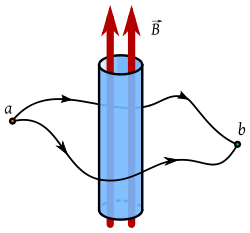
\includegraphics[scale=0.6]{Immagini/aharonov_bohm.png}
    \caption{Illustrazione del setup dell'effetto Aharonov-Bohm}
    \label{fig:aharonov_bohm}
\end{figure}%Ricontrollare [TO DO]

\subsubsection{Fase di Berry}
Lo sfasamento che acquisisce una $\psi$ dopo un \textit{ciclo} è detto \textbf{fase di Berry}, e per $\psi$ normalizzate ($\braket{\psi|\psi} = 1$) ha la seguente definizione:
\[
e^{\oint_{\mathcal{C}}{\left\langle\psi\right|d\psi\rangle\ }}
\]
dove $\mathcal{C}$ è una famiglia di funzioni d'onda "sfasate" (vedi sotto).\\
Con questa definizione la fase di Berry è un'osservabile. Mostriamo che il suo valore è non nullo se calcolata lungo un percorso ciclico (per esempio una circonferenza).\\
%[Done] (correggere negli appunti vecchi la i nella fase di Berry) OK
Partiamo considerando:
\[
\psi_n\left(x\right)=\frac{1}{\sqrt{2\pi}}e^{i\left(n+\frac{\gamma}{2\pi}\right)x}
\]
Le $\psi_n$ sono definite a meno di una fase "attorno al cerchio", ossia a meno di una $\psi_\alpha(x)$:
\[
\{\psi_\alpha(x)\>|\>\psi_{2\pi}(x) = e^{i\gamma} \psi_0(x)\}; \quad \alpha \in [0,2\pi[
\]
Giungiamo quindi alla famiglia:
\[
\psi_{n,\alpha}=\frac{1}{\sqrt{2\pi}}e^{i\left(n+\frac{\gamma}{2\pi}\right)\left(x+\alpha\right)}; \quad \psi_{n,2\pi}(x) = e^{i\gamma}\psi_{n,0}(x); \quad \alpha \in [0,2\pi [
\]
Possiamo ora definire $\mathcal{C}$:
\[
C=\psi_{n,\alpha}\left(x\right)\>|\>  \psi_{n,2\pi}\left(x\right)=e^{i\gamma}\psi_{n,0}(x)
\]
e quindi calcolare l'integrale per la fase di Berry:
\begin{align*}
\oint_{\mathcal{C}}{\left\langle\psi_{n,\alpha}\right|d\psi_{n,\alpha}\rangle}&=\int_{0}^{2\pi}{d\alpha\ \left\langle\psi_{n,\alpha}\ \right|\frac{d}{d\alpha}\psi_{n,\alpha}\rangle\ }\\
\left\langle\psi_{n,\alpha}\ \right|\frac{d}{dx}\psi_{n,\alpha} \rangle &=\int_{0}^{2\pi}{dx\ \frac{1}{2\pi}\ e^{-i\left(\frac{\gamma}{2\pi}+n\right)\left(x+\alpha\right)}\left(i\left(\frac{\gamma}{2\pi}+n\right)\right)e^{i\left(\frac{\gamma}{2\pi}+n\right)\left(x+\alpha\right)\ }}=i\left(\frac{\gamma}{2\pi}+n\right)\\
e^{\oint_{\mathcal{C}}\left\langle\psi\middle| d\psi\right\rangle}&=\exp{\int_{0}^{2\pi}{d\alpha\ i\left(\frac{\gamma}{2\pi}+n\right)}}=\exp{i\ 2\pi\left(\frac{\gamma}{2\pi}+n\right)}=e^{i\gamma} 
\end{align*}

\section{Stati misti in MQ}
Supponiamo di non conoscere in quale stato puro $\ket{\phi}$ il sistema si trovi, ma solo di sapere che può essere negli stati puri $\left|\phi_1\right\rangle,\dots, |\phi_n\rangle $ (che consideriamo normalizzati, $\braket{\phi_i|\phi_i}=1$) con probabilità $p_1\dots p_n$, $\sum_{i=1}^{n}p_i=1$.\\
\textbf{Nota}: $n$ è per forza numerabile, ma le $\phi$ non hanno vincoli di ortogonalità, e le $p_i$ sono probabilità classiche.\\
Dalle regole della probabilità, se $\Sigma$ denota lo stato di informazione non massimale (misto) sopra descritto e $A$ è un'osservabile, allora il valor medio di A nello stato $\Sigma$ è dato da una "media pesata" dei valor medi dei singoli stati puri:
\[
\langle A \rangle_\Sigma = \sum_{i=1}^n p_i\bra{\phi_i}A\ket{\phi_i}
\]
Osserviamo che se $\phi$ è un qualsiasi stato di $\hs$, possiamo scrivere il valor medio come:\marginpar{Valor medio in termini di traccia}
\[
\left\langle\phi\left|A\right|\phi\right\rangle
=\op{Tr}(\ket{\phi}\bra{\phi}A)
\]
Infatti, sia $\left\{\left|\chi_j\right\rangle,\
j=1,\ldots,\dim{\mathcal{H}}\right\}$ una base ON per $\hs$, con la condizione che $\left|\chi_1\right\rangle=\ket{\phi}$ (allineo il primo vettore della base con il vettore in esame). Allora:
\[
\op{Tr}(\ket{\phi}\bra{\phi}A) = \sum_{j=1}^{\op{dim}\hs}\bra{\chi_j}(\ket{\phi}\bra{\phi}A)\ket{\chi_j} \underset{(a)}{=} \sum_{j=1}^{\op{dim}\hs}\delta_{ji}\bra{\phi}A\ket{\chi_j} = \bra{\phi}A\ket{\phi}
\]
dove in (a) si è usato il fatto che $\left\langle\chi_j\middle|\phi\right\rangle=\left\langle\chi_j\middle|\chi_1\right\rangle=\delta_{j1}$ per l'ortonormalità (essendo $\ket{\phi}$ perpendicolare a tutti i $\ket{\chi_j}$ e parallelo al primo per costruzione).
\begin{mdframed}[hidealllines=true,backgroundcolor=green!20,innerleftmargin=3pt,innerrightmargin=3pt,leftmargin=-3pt,rightmargin=-3pt]
\textbf{Nota}: in uno spazio di Hilbert\index{Traccia} $\hs$, con $\ket{\chi_j}$ base ON, la \textbf{traccia} è definita come:
\[
\op{Tr}(\cdot) = \sum_j \bra{\chi_j} (\cdot) \ket{\chi_j}
\]
Ed è indipendente dalla scelta della base.\\
In effetti, nel caso finito dimensionale di $\mathbb{R}^n$, se si parte da una base canonica si ritrova la somma degli elementi sulla diagonale principale.\\
Dalla definizione segue anche che la traccia è \textbf{lineare}.
\end{mdframed}
Sostituendo questo risultato nella formula della media:
\[
\langle A \rangle_\Sigma = \sum_{i=1}^n p_i \bra{\phi_i}A\ket{\phi_i} = \sum_{i=1}^n p_i \op{Tr}(\ket{\phi_i}\bra{\phi_i}A) \underset{(a)}{=} \op{Tr}\left( \hlc{Yellow}{\sum_{i=1}^n p_i \ket{\phi_i}\bra{\phi_i}A}\right )
\]
dove in (a) si è usata la linearità della traccia.\\
Il termine evidenziato è detto \textbf{matrice densità}:\marginpar{Matrice di densità}\index{Matrice densità}
\[
\rho \equiv \sum_{i=1}^{n}{p_i\left|\phi_i\right\rangle\langle\phi_i|}
\]
Dalla sua definizione segue che: \marginpar{Proprietà della matrice densità}
\begin{enumerate}
    \item $\rho$ è simmetrico\marginpar{$\rho$ è simmetrico}, ossia $\displaystyle \rho = \rho^\dag$, in quanto $A$ è autoaggiunto, $p_i$ è reale e $\left(\middle|\phi\right\rangle{\left\langle\phi\middle|\right)}^\dag=\left|\phi\right\rangle\left\langle\phi\right|$
	\item $\rho$ è \textbf{positivo}\marginpar{$\rho$ è positivo} ($\rho \geq 0$), cioè produce solo "valor medi positivi": $\forall \psi \left\langle\psi\right|\rho \ket{\psi}\geq 0$. Infatti:
	\begin{align*}
	    \left\langle\psi\left|\rho\right|\psi\right\rangle&=\sum_{i}p_i\left\langle\psi\middle|\phi_i\right\rangle\left\langle\phi_i\middle|\psi\right\rangle=
	    \sum_i p_i \braket{\psi|\phi_i}(\braket{\psi|\phi_i})^* =
	    \\
	    &=\sum_{i}p_i\left|\left\langle\psi\middle|\phi_i\right\rangle\right|^2\geq0; \quad \forall \ket{\psi}\in \hs
	\end{align*}
	(Dalla positività si ha poi subito che è autoaggiunto, come nel caso di un numero complesso, che è positivo solo se reale)
	\item $\displaystyle \op{Tr}\rho = 1$, infatti \marginpar{$\op{Tr} \rho = 1$} $\op{Tr}(\ket{\phi}\bra{\phi}) = \sum_j \braket{\chi_j|\phi}\braket{\phi|\chi_j} = |\braket{\phi|\phi}|^2 = 1$ (essendo $\ket{\chi_1} = \ket{\phi}$). Sfruttando allora la linearità della traccia, e il fatto che le $p_i$, esaurendo tutte le possibilità, si sommano a $1$ (cosa che avevamo chiesto fin dal principio):
	\[
	\op{Tr}\left(\sum_i p_i \ket{\phi_i}\bra{\phi_i}\right) = \sum_i p_i \op{Tr}(\ket{\phi_i}\bra{\phi_i}) = \sum_i p_i = 1
	\]
\end{enumerate}
\begin{dfn}\marginpar{Descrizione matematica di uno stato}
Uno \textbf{stato} (misto o puro) in MQ è descritto da un operatore $\rho$ che soddisfa 1-3.
\end{dfn}
Gli \textbf{stati puri} sono descritti dalle $\rho$ che soddisfano $\rho =\rho^2$. In tal caso $\rho$  è un proiettore, ma poiché la traccia di $\rho$ deve fare $1$, deve essere unidimensionale (cioè c'è un solo $p_i=1$ e tutti gli altri sono $0$, poiché solo i numeri $0$ e $1$ sono uguali al loro quadrato\footnote{In particolare, se ci fosse un $p_i \neq 0,1$ allora non si avrebbe $\rho = \rho^2$, e se vi fossero più di un $p_i$ pari a $1$ allora $\op{Tr}\rho > 1$, e nel caso non ve ne fosse nessuno $\op{Tr}\rho = 0$, che va contro alla definizione di matrice di densità}).\\
Ma allora in tal caso la somma è ridotta a un solo elemento (tutti gli altri sono annullati dalle $p_i = 0$), e quindi $\rho =\ket{\psi}\bra{\psi}$ per un qualche $\ket{\psi}\in \hs$ normalizzato  ($\braket{\psi|\psi}=1$).\\
Ci si potrebbe allora chiedere\marginpar{$\rho$ $\leftrightarrow$ raggi vettori} se $\rho$, visto che è definito in termini di $\ket{\psi}\in \hs$ - che sono definiti a meno di una fase - presenti la stessa ambiguità. Ma se $\rho$ è la descrizione di uno stato, che è dato da un raggio vettore in $\mathcal{S}$, tale ambiguità deve sparire. E infatti, si verifica che:
\begin{align*}
    \ket{\psi}&\rightarrow e^{i\alpha}\ket{\psi}\\
\rho &\rightarrow e^{i\alpha}\ket{\psi}\bra{\psi}e^{-i\alpha}=\ket{\psi}\bra{\psi}
\end{align*}
Ma allora $\rho^2=\rho$ sono in corrispondenza biunivoca con i raggi vettori dello spazio di Hilbert.\\
Ciò è comodo sperimentalmente, perché $\rho$ costituisce un'osservabile ( e qui potenzialmente può essere misurata).\\
Per esempio, in un sistema di due fotoni, lo stato delle polarizzazioni è una matrice $2\times 2$ di numeri che si possono ricavare sperimentalmente. Perciò, per verificare se un sistema creato in laboratorio sia in uno stato puro o meno, basta determinare tale matrice $A$, calcolarne il quadrato e vedere se viene lo stesso risultato di partenza, ossia se si ha $A^2 = A$.\\

Vediamo che, come nel caso classico, uno stato misto quantistico può essere scritto come una combinazione \textit{convessa}\footnote{Una combinazione convessa è una combinazione lineare di elementi fatta con coefficienti non negativi a somma $1$. Per esempio: $\lambda_1 x_1 + \dots +\lambda_m x_m$ è convessa se $\lambda_i \geq 0$ per $i=1,\dots,m$ e $\sum_{i=1}^m \lambda_i = 1$} di stati puri, scritti come proiettori.\\
\textbf{Attenzione}: partendo dalla decomposizione di $\ket{\psi} = \ket{\psi_1}+\ket{\psi_2}$ si potrebbe essere tentati di scrivere la seguente relazione per la sovrapposizione di stati:
\[
|\psi_1\rangle \langle \psi_1|+\left|\psi_2\right\rangle\left\langle\psi_2\right|\neq \ket{\psi}\bra{\psi}
\]
Ma tale uguaglianza non è corretta. In effetti il primo membro è (a meno di una normalizzazione) la matrice densità di uno \textit{stato misto}, mentre il secondo è ovviamente uno \textit{stato puro} (essendo costituito da \textit{un solo} proiettore).\\
Matematicamente la faccenda risulta evidente prendendo $\ket{\psi_1}$ e $\ket{\psi_2}$ ON. Allora le espressioni del membro a sinistra sono per forza matrici diagonali, ma quella a destra generalmente non lo è.\\
Concretamente, siano per esempio (trascurando, di nuovo, le normalizzazioni):
\begin{align*}
\ket{\psi_1}&=\begin{pmatrix}
1\\
0
\end{pmatrix};\>\ket{\psi_2} = \begin{pmatrix}
0\\
1
\end{pmatrix};\>\ket{\psi}=\ket{\psi_1}+\ket{\psi_2}=\begin{pmatrix}
1\\
1
\end{pmatrix}\\
\ket{\psi_1}\bra{\psi_1} + \ket{\psi_2}\bra{\psi_2} &= 
\begin{pmatrix}
1\\
0
\end{pmatrix}
\begin{pmatrix}
1 & 0
\end{pmatrix}
+
\begin{pmatrix}
0\\
1
\end{pmatrix}
\begin{pmatrix}
0 & 1
\end{pmatrix} =
\begin{pmatrix}
1 & 0\\
0 & 0
\end{pmatrix}
+ \begin{pmatrix}
0 & 0\\
0 & 1
\end{pmatrix}
= \begin{pmatrix}
1 & 0\\
0 & 1
\end{pmatrix}\\
\ket{\psi}\bra{\psi} &=
\begin{pmatrix}
1\\
1
\end{pmatrix}
\begin{pmatrix}
1 & 1
\end{pmatrix}
=
\begin{pmatrix}
1 & 1\\
1 & 1
\end{pmatrix}
\end{align*}
Si nota quindi che nell'espressione del membro a sinistra mancano tutti i termini fuori dalla diagonale.\\

Nel caso \textbf{classico} possiamo scrivere uno stato come combinazione convessa (non numerabile) di stati puri:
\[
\rho \left(q,p\right)=\int dq_0\,dp_0 \rho \left(q_0,p_0\right) \underbrace{\delta \left(q-q_0\right)\delta \left(p-p_0\right)}_{\text{Stati puri}}
\]
È quindi ben definita (dalla $\rho(q,p)$) la \textit{famiglia} degli stati puri che definiscono lo stato misto.\\
In MQ la situazione è diversa. Dall'autoaggiuntezza di $\rho$  ($\rho = \rho^\dag$) si ha che esistono autovettori $\ket{\lambda_n}$ di $\rho$ che formano una base ON. Possiamo allora
decomporre $\rho$ spettralmente:
\[
\rho =\sum_{n}{\lambda_n|\lambda_n\rangle\langle\lambda_n|};\quad \op{Tr}\left(\rho\right)=1= \sum_{n}\lambda_n
\]
Abbiamo allora ottenuto una descrizione completamente equivalente a quella che abbiamo finora usato:
\[
\rho = \sum_{i}{p_i|\phi_i\rangle\langle\phi_i|}
\]
in cui, tra l'altro, le $\ket{\phi_i}$ non devono neppure essere ON.\\
Perciò si hanno famiglie \textit{diverse} di stati puri che danno la stessa informazione dello stato misto!\\
In MC posso comunque sapere gli stati puri da cui parto - non so la loro combinazione esatta), ma in MQ in uno stato misto non è chiara neanche la famiglia di stati puri sottostante (è un livello decisamente più profondo di ignoranza).
\end{document}